در این پوشه تمام اطلاعات گیت‌هاب قرار دارد

\begin{figure}[H]
	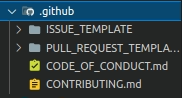
\includegraphics[width=.3\textwidth]{Folders-Files/github.png}
	\centering
	\caption{ساختار قرارگیری گیت‌هاب}
	\label{fig:folder-github}
\end{figure}


\paragraph{پوشه \LR{ISSUE TEMPLATE}}
در این پوشه قالب ایجاد مسئله شامل خطا، باگ و ... در گیت‌هاب قرار دارد.

\paragraph{پوشه \LR{PULL REQUEST TEMPLATE}}
در این پوشه قالب ایجاد درخواست ادغام در گیت‌هاب قرار دارد.

\paragraph{فایل \LR{CODE OF CONDUCT}}
در این فایل نحوه مشارکت در پروژه تعریف شده است.

\paragraph{فایل \LR{CONTRIBUTING}}
در این فایل مشارکت‌کنندگان در پروژه تعریف شده‌اند.
